\documentclass[12pt]{article}
\usepackage{graphicx}
\usepackage{float}
\usepackage{lipsum}
\usepackage{fancyhdr}
\usepackage{hyperref}
\usepackage{listings}
\usepackage{xcolor}

% Define custom colors for code listing
\definecolor{codegray}{gray}{0.9}

% Define style for C code
\lstdefinestyle{CStyle}{
    language=C,
    backgroundcolor=\color{codegray},
    basicstyle=\footnotesize\ttfamily,
    breaklines=true,
    frame=single,
    numbers=left,
    numberstyle=\tiny\color{gray},
    keywordstyle=\color{blue},
    commentstyle=\color{teal},
    stringstyle=\color{red},
}

\fancypagestyle{firstpage}{
    \fancyhf{}
    \renewcommand{\headrulewidth}{0pt}
    \fancyfoot[R]{Francesco Porritiello 0124002486 \\ Francesco Esposito 0124002629}
}

\begin{document}

\thispagestyle{firstpage}

\begin{figure}[H]
\centering

\includegraphics[width=0.50\linewidth]{logo.PNG}

\vspace{1cm}

{\Huge \textbf{Università degli studi di Napoli “PARTHENOPE”}}

\vspace{1cm}

{\Huge \textbf{Reti di Calcolatori}}

\vspace{1cm}

{\Large \textbf{Traccia - Università}}

\vspace{4cm}

{\textbf{Anno 2024/2025}}

\end{figure}

\newpage

\tableofcontents
\newpage

\section{Introduzione}
\subsection{Obiettivo}
Scrivere un'applicazione client/server parallelo per gestire gli esami universitari.

\begin{itemize}
    \item \textbf{Studente}
    \begin{enumerate}
        \item Chiede alla segreteria se ci siano esami disponibili per un corso.
        \item Invia una richiesta di prenotazione di un esame alla segreteria.
    \end{enumerate}
    \item \textbf{Segreteria}
    \begin{enumerate}
       \item Inserisce gli esami sul server dell'università (salvare in un file o conservare in memoria il dato).
       \item Inoltra la richiesta di prenotazione degli studenti al server universitario.
       \item Fornisce allo studente le date degli esami disponibili per l'esame scelto dallo studente.
    \end{enumerate}
    \item \textbf{Università}
    \begin{enumerate}
       \item Riceve l'aggiunta di nuovi esami.
       \item Riceve la prenotazione di un esame.
       \item Ad ogni richiesta di prenotazione invia alla segreteria il numero di prenotazione progressivo assegnato allo studente e la segreteria a sua volta lo inoltra allo studente.
    \end{enumerate}
\end{itemize}

\newpage

\section{Descrizione}
Il sistema è costituito da tre entità, Studente, Segreteria ed Università.\newline\newline
Essi fanno uso dell'architettura client/server sfruttando il protocollo TCP/IP per la comunicazione.

\subsection{Architettura}
Server e Segreteria fungono entrambi sia da client che da server, mentre lo Studente soltanto da client.\newline\newline
L'Università comunica in modo diretto esclusivamente con la Segreteria; quest'ultima viene usata come intermediara dallo Studente per effettuare richieste all'Università.\newline\newline La sequenza con cui il sistema deve essere avviato è la seguente:
\begin{enumerate}
    \item Server
    \item Segreteria
    \item Studente\newline
\end{enumerate}
Il Server Universitario, una volta avviato, attende che la Segreteria si connetta. Stabilita la connessione, la Segreteria, può adesso effettuare richieste all'Università, restando allo stesso tempo in attesa di connessioni da parte del client Studente per servire le sue richieste.

\begin{figure}[H]
\centering
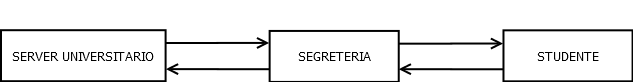
\includegraphics[width=1.00\linewidth]{Schema.PNG}
\end{figure}

\section{Use-Case}

\begin{figure}[H]
\centering
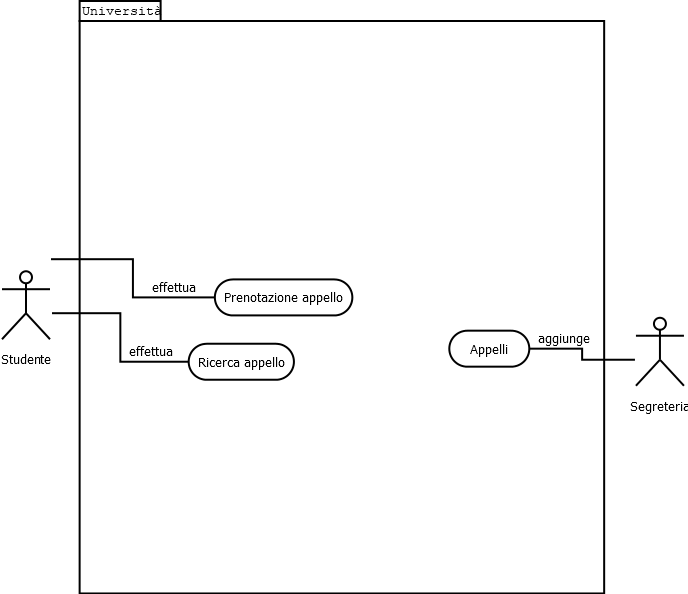
\includegraphics[width=1.00\linewidth]{Use2.PNG}
\end{figure}

\newpage

\section{Componenti del Sistema}
\begin{itemize}
    \item Studente - Fornisce un'interfaccia a linea di comando per:
    \begin{enumerate}
        \item Ricerca Appelli.
        \item Prenotazione Appelli.
            \newline
    \end{enumerate}
    \item Segreteria - Si occupa di:
    \begin{enumerate}
        \item Aggiungere Appelli.
        \item Gestire le richieste dello Studente mediando con l'Università quando effettua operazioni di ricerca e/o prenotazione appelli.
            \newline
    \end{enumerate}
    \item Università - Si occupa di:
    \begin{enumerate}
        \item Fornire le date degli Appelli disponibili.
        \item Salvare in un file gli Appelli aggiunti.
        \item Salvare in un file le prenotazioni agli Appelli.
        \item Inoltrare il numero di prenotazione progressivo ad uno Studente che ha effettuato una prenotazione ad un Appello.         
    \end{enumerate}
    
\end{itemize}

\newpage

\section{Dettagli implementativi}
Di seguito verranno descritti i dettagli implementativi del sistema:

\begin{itemize}
    \item Università
    \item Segreteria
    \item Studente
\end{itemize}

\subsection{Università}

\begin{lstlisting}[style=CStyle]
void gestisciRichiesta(int client_socket) {
    char buffer[BUFFER_SIZE] = {0};        // Lettura dei dati dal client
    char tipo_richiesta;                   // Tipi di richieste ('A', 'P', 'I')
    char nome_esame[BUFFER_SIZE] = {0};    // Nome esame
    char data_esame[BUFFER_SIZE] = {0};    // Data esame
    char linea[BUFFER_SIZE] = {0};         // Buffer per leggere la linea del file
    int esame_trovato = 0;                 // Flag per verificare se un esame e' trovato

    // Leggi la richiesta dal client
    read(client_socket, buffer, BUFFER_SIZE);
    tipo_richiesta = buffer[0]; // La prima lettera indica il tipo di richiesta

    if (tipo_richiesta == 'A') { // Aggiunta di un esame
        // Prendi tutto il contenuto fino alla newline
        sscanf(buffer + 1, "%[^\n]", buffer); 
        
    // Trova la posizione dell'ultimo spazio, che separa il nome dell'esame dalla data
    char *space_pos = strrchr(buffer, ' ');
    
    if (space_pos != NULL) {
        // Calcola la lunghezza del nome dell'esame e copia il nome
        int nome_len = space_pos - buffer;                
        strncpy(nome_esame, buffer, nome_len);
        nome_esame[nome_len] = '\0'; // Aggiunge il terminatore
        
        // Copia la data dell'esame
        strcpy(data_esame, space_pos + 1);
    }

        // Apri il file degli esami sia per la lettura che per la scrittura
        FILE *file = fopen(EXAMS_FILE, "r+");
        if (file == NULL) {
            perror("Errore nell'apertura del file esami");
            exit(EXIT_FAILURE);
        }

        // Crea un file temporaneo per scrivere i dati aggiornati
        FILE *temp_file = fopen("temp.txt", "w");
        if (temp_file == NULL) {
            perror("Errore nell'apertura del file temporaneo");
            fclose(file);
            exit(EXIT_FAILURE);
        }

        // Leggi il file degli esami riga per riga
        while (fgets(linea, sizeof(linea), file)) {
            char esame[BUFFER_SIZE] = {0};
            sscanf(linea, "%[^\n]", esame); // Prendi il nome dell'esame

            if (strstr(esame, nome_esame) == esame) {
                // Esame gia' esistente, aggiungi la nuova data
                fprintf(temp_file, "%s %s\n", esame, data_esame);
                esame_trovato = 1;
            } else {
                // Copia la riga esistente nel file temporaneo
                fprintf(temp_file, "%s", linea);
            }
        }

        // Se l'esame non e' stato trovato, aggiungilo
        if (!esame_trovato) {
            fprintf(temp_file, "%s %s\n", nome_esame, data_esame);
        }

        // Chiudi i file 
        fclose(file);
        fclose(temp_file);
        // Sostituisci il file originale con quello temporaneo
        remove(EXAMS_FILE);
        rename("temp.txt", EXAMS_FILE);

        // Invia al client una conferma che l'esame e' stato aggiunto
        send(client_socket, "Esame aggiunto con successo.\n", 29, 0);
    } else if (tipo_richiesta == 'P') { // Se la richieta e' quella di prenotazione
    
        sscanf(buffer + 1, "%[^\n]", buffer);

        // Apri il file delle prenotazioni
        FILE *file = fopen(BOOKINGS_FILE, "a");
        if (file == NULL) {
            perror("Errore nell'apertura del file prenotazioni");
            exit(EXIT_FAILURE);
        }

        // Genera un numero di prenotazione casuale tra 1 e 100
        int numero_prenotazione = rand() % 100 + 1;

        // Aggiungi la prenotazione al file
        fprintf(file, "%s \n", buffer);
        fclose(file);

        // Invia la risposta al client
        char risposta[BUFFER_SIZE] = {0};
        snprintf(risposta, sizeof(risposta), "Prenotazione - %s. Numero prenotazione: %d\n", buffer, numero_prenotazione);
        send(client_socket, risposta, strlen(risposta), 0);
        
    } else if (tipo_richiesta == 'I') { // Richiesta per infromazioni su un esame
        sscanf(buffer + 1, "%[^\n]", nome_esame);

        // Apri il file degli esami in modalita' lettura
        FILE *file = fopen(EXAMS_FILE, "r");
        if (file == NULL) {
            perror("Errore nell'apertura del file esami");
            exit(EXIT_FAILURE);
        }

        // Cerca l'esame nel file
        while (fgets(linea, sizeof(linea), file)) {
            if (strstr(linea, nome_esame) != NULL) {
                send(client_socket, linea, strlen(linea), 0); // Invia la riga al client
                esame_trovato = 1; // Segna che l'esame e' stato trovato
            }
        }
        fclose(file);
        // Se l'esame non e' stato trovato, invia un messaggio al client
        if (!esame_trovato) {
            send(client_socket, "Esame non trovato.\n", 19, 0);
        }
    }
}
\end{lstlisting}

La funzione \textbf{gestisciRichiesta}, legge i dati dal client segreteria e determina il tipo di richiesta (\textbf{A}: aggiunta, \textbf{P}: prenotazione, \textbf{I}: informazioni).

A seconda del tipo di richiesta, esegue operazioni appropriate.

\newpage

\subsection{Segreteria}

\begin{lstlisting}[style=CStyle]
void* gestisciRichiesta(void* arg) { // Funzione che gestisce le richieste effettuate dallo Studente.
    int client_socket = *(int*)arg; // Assegnazione della socket client.
    free(arg);

    char buffer[BUFFER_SIZE] = {0}; // Buffer per l'inoltro delle richieste.
    char risposta[BUFFER_SIZE] = {0}; // Buffer che conterra' la risposta del server Universitario per lo Studente.
    int sock_universita; // Socket server universitario.
    struct sockaddr_in server_addr_universita; // Definisce una struttura sockaddr_in per memorizzare l'indirizzo del server dell'universita'.

    // Leggi la richiesta dallo studente.
    if (read(client_socket, buffer, BUFFER_SIZE) < 0) {
        perror("Errore nella lettura della richiesta");
        close(client_socket);
        pthread_exit(NULL);
    }

    // Creazione del socket per la connessione con il server universitario.
    if ((sock_universita = socket(AF_INET, SOCK_STREAM, 0)) < 0) {
        perror("Errore nella creazione del socket per il server universitario");
        close(client_socket);
        pthread_exit(NULL);
    }

    server_addr_universita.sin_family = AF_INET; // Imposta la famiglia di indirizzi su AF_INET, specificando che si utilizzera' il protocollo IPv4.
    server_addr_universita.sin_port = htons(SERVER_PORT); // Imposta il numero di porta del server, convertendolo in network byte order con htons.

    if (inet_pton(AF_INET, SERVER_IP, &server_addr_universita.sin_addr) <= 0) { // Converte l'indirizzo IP del server da stringa a formato binario e lo memorizza nella struttura sockaddr_in.
        perror("Indirizzo non valido o non supportato");
        close(client_socket);
        pthread_exit(NULL);
    }

    // Connessione al server universitario.
    if (connect(sock_universita, (struct sockaddr *)&server_addr_universita, sizeof(server_addr_universita)) < 0) {
        perror("Connessione al server universitario fallita");
        close(client_socket);
        pthread_exit(NULL);
    }

    // Invia la richiesta al server universitario.
    if (send(sock_universita, buffer, strlen(buffer), 0) < 0) {
        perror("Errore nell'invio della richiesta al server universitario");
        close(sock_universita);
        close(client_socket);
        pthread_exit(NULL);
    }

    // Ricevi la risposta dal server universitario.
    int len = read(sock_universita, risposta, BUFFER_SIZE);
    if (len < 0) {
        perror("Errore nella lettura della risposta dal server universitario");
        risposta[0] = '\0'; // Risposta vuota in caso di errore.
    } else {
        risposta[len] = '\0';
    }

    // Invia la risposta del server universitario allo studente.
    if (send(client_socket, risposta, strlen(risposta), 0) < 0) {
        perror("Errore nell'invio della risposta allo studente");
    }

    close(sock_universita); // Chiusura delle socket.
    close(client_socket);

    pthread_exit(NULL); // Termina il thread corrente e restituisce un valore di uscita NULL.
}
\end{lstlisting}

La funzione \textbf{gestisciRichiesta}, gestisce le richieste dello studente, per poi inviarle al server universitario. Si occupa poi di inoltrare la risposta ricevuta dal server universitario allo studente.

\subsection{Studente}

\begin{lstlisting}[style=CStyle]
void inviaRichiestaAllaSegreteria(char tipoRichiesta, char *matricola, char *nomeEsame, char *dataEsame) { // Funzione per la gestione della richiesta degli appelli disponibili.
    int sock_segreteria; // Socket della segreteria.
    struct sockaddr_in server_addr_segreteria; // Indirizzo della Segreteria.
    char buffer[BUFFER_SIZE] = {0}; 

    // Creazione del socket per la connessione con la segreteria
    if ((sock_segreteria = socket(AF_INET, SOCK_STREAM, 0)) < 0) {
        perror("Errore nella creazione del socket");
        exit(EXIT_FAILURE);
    }

    server_addr_segreteria.sin_family = AF_INET; // Si specifica che l'indirizzo del server utilizzera' l'indirizzamento ipv4.
    server_addr_segreteria.sin_port = htons(SECRETARY_PORT); // Converte il numero di porta della Segreteria.

    if (inet_pton(AF_INET, SERVER_IP, &server_addr_segreteria.sin_addr) <= 0) { // Conversione dell'indirizzo IP del server da formato testuale a formato binario.
        perror("Indirizzo non valido o non supportato");
        exit(EXIT_FAILURE);
    }

    // Connessione alla segreteria
    if (connect(sock_segreteria, (struct sockaddr *)&server_addr_segreteria, sizeof(server_addr_segreteria)) < 0) {
        perror("Connessione fallita");
        exit(EXIT_FAILURE);
    }

    // Invia la richiesta alla segreteria.
    if (tipoRichiesta == 'P') {
        snprintf(buffer, sizeof(buffer), "%c%s %s %s", tipoRichiesta, matricola, nomeEsame, dataEsame); // Viene inserito nel buffer la tipologia della richiesta, Esame e Data esame. 
    } else {
        snprintf(buffer, sizeof(buffer), "%c%s", tipoRichiesta, nomeEsame); // Viene inserito nel buffer la tipologia della richiesta ed il nome esame,
    }

    send(sock_segreteria, buffer, strlen(buffer), 0); // Invio dei dati contenuti in buffer alla Segreteria.

    // Lo studente riceve risposta dell'opportuna richiesta fatta.
    int len = read(sock_segreteria, buffer, BUFFER_SIZE);
    if (len > 0) {
        buffer[len] = '\0';
        printf("%s\n", buffer);
    }

    close(sock_segreteria); //Chiusura della connessione con la Segreteria.
}
\end{lstlisting}

La funzione \textbf{inviaRichiestaAllaSegreteria}, si occupa dell'invio di richieste alla segreteria.

\newpage

\section{Compilazione ed Esecuzione}
Di seguito verranno mostrati i comandi per compilare ed eseguire il sistema su piattaforme *Unix-Like.
\begin{itemize}
    \item Università
    \begin{enumerate}
        \item Compilazione: "gcc server.c -o server"
        \item Esecuzione: "./uni"\newline
    \end{enumerate}
    \item Segreteria
    \begin{enumerate}
        \item Compilazione: "gcc segre.c -o segre"
        \item Esecuzione: "./segre"\newline
    \end{enumerate}
    \item Studente
    \begin{enumerate}
        \item Compilazione: "gcc stu.c -o stu"
        \item Esecuzione: "./stu"\newline
    \end{enumerate}
\end{itemize}
* Non possono essere compilati ed eseguiti su sistemi operativi Windows in quanto sono stati pensati per sfruttare librerie e system-call POSIX.

\end{document}